\chapter{Architecture of a Quantum Computer}

Although the challenges of building a fault-tolerant qubit have by no means been met, the field is rapidly reaching the point where
it is possible to start running algorithms on quantum computers. While algorithms such as Shor's algorithm for prime factorization
would require $2N + 3$ logical qubits with an arbitrarily long lifetime~\cite{Beauregard:2003,6657074}, other algorithms may
be able to achieve a quantum speedup with a limited number of noisy qubits. Algorithms and systems operating in this regime are
said to be in the Noisy Intermediate-Scale Quantum (NISQ) regime~\cite{Preskill2018quantumcomputingin}, a term coined by John Preskill
in 2018 to distinguish between a full-scale quantum computer, with a large number of error corrected qubits, and one that we may realize
in the coming decade, containing as few 10s of noisy, imperfect qubits. In the near term, the race is on to achieve \textbf{quantum supremacy},
a calculation on a quantum computer whose simulation on a classical computer is intractable. The expectation is that this milestone will
be beaten in the coming years, with a system of approximately 50 noisy qubits~\cite{s41567-018-0124-x}. Based on the current state of the field
this will likely occur using superconducting transmon-like qubits solving a model problem such as Boson sampling~\cite{Aaronson:2011}. While such a
result would certainly be groundbreaking, the more interesting result would be a demonstration of \textbf{quantum advantage}, an algorithm whose simulation on a
classical computer is intractable, but one which also solves a useful problem. While Boson sampling certainly seems to be a classically hard problem,
the solution it provides does not seem to be one that has many practical implications. In the near term, our best bet for achieving a useful result
seems to be using the Variational Quantum Eigensolver algorithm \cite{ncomms5213}, which, as we alluded to in the introduction of Chapter~\ref{sec:quest}, would allow us
to model molecules that we could not on a classical computer, with a small number (100s) of imperfect qubits~\cite{PhysRevA.92.042303}.
To date, several experimental realizations of this algorithm have been published~\cite{nature23879,PhysRevX.8.011021,10.1038/s41586-019-1040-7},
although none have yet simulated a molecule that is classically intractable.

\section{Designing an Architecture}
Given the rapid progression of the field, the questions surrounding architecting a quantum computer have been gaining increasing attention,
particularly as the number of qubits grows beyond the limits that we might control with a ad-hoc architecture that a single graduate student might construct.
The challenge for experimentalists continues to come down to building scaleable building blocks, which balance the need for experimental
flexibility surrounding qubits whose designs and control requirements remain in flux, but whose footprint does not explode for larger numbers
of physical qubits. Thankfully, at least within the realm of solid-state qubits (that is superconductor and semiconductor based qubits),
there is substantial overlap in the requirements for control and readout of qubits, that allows us to design architectures for hypothetical
quantum machines. Let's therefore enumerate a number of requirements for a control and readout architecture controlling a solid-state qubit:
\begin{itemize}
  \item Cryogenic operation: Solid-state qubits must be operated in cryogenic environments, stemming from the requirement that the thermal energy should be well below the level spacing of energy levels in the qubit, as well as the need for superconducting elements in some designs. Any control and readout architecture must, therefore, be low power, and avoid carrying thermal energy or noise down to the qubit device.
  \item Control fidelity: In order to reach the fault-tolerance threshold, fidelities of individual qubits must exceed $99\%$, and should ideally be well above the $(1 - 10^{-5})$ level to avoid prohibitive error correction requirements~\cite{6657074}. Depending on the rotation rate and decoherence rates of individual qubits, control lines must have bandwidths of several 10's of \si{\giga\hertz}, along with high density, low crosstalk and low noise.
  \item Readout fidelity: Readout of qubits brings unique challenges, requiring low probe powers in order to avoid disturbing the state while it is being measured, and limited measurement time due to decoherence. In addition, QEC in general requires the continued measurement of ancilla qubits while nearby qubits are operational, leading to stringent crosstalk requirements. In order to obtain a sufficient signal-to-noise ratio, cryogenic amplification is generally required, which in turn limits and scaleable design to one, or a few, readout lines. As such, some form of multiplexing, either frequency-domain or time-domain, is necessary for readout.
  \item Space: This requirement is particularly difficult to accomplish as it occurs over three orders of magnitude over the scale of the chip, the cryostat and at room temperature. Each of these are discussed in detail below, but we state the problem briefly here. On a chip scale, dense control lines must be fit into an area set by the distance over which we can achieve coupling between qubits, setting micron-scale limits on on-chip structures. On a cryostat level, the need to operate at \si{\milli\kelvin} in a cryostat places centimeter-scale limits on cryogenic components. Finally at room temperature, phase matching of control pulses and the need for active feedback places limits on the size of the instrumentation used to control individual qubits.
\end{itemize}

\afterpage{
  \clearpage
  \thispagestyle{empty}
  \begin{landscape}
  \begin{table}
    \centering
    \def\arraystretch{1.5}
    \begin{tabular}{|l|l|l|l|l|l|l|}
    \hline
    \multicolumn{3}{|l|}{} & \shortstack{CryoCMOS Architecture\\(Section~\ref{sec:gooseberry})} & \shortstack{Prime-Lines Architecture\\(Section~\ref{sec:primelines})} & \shortstack{Frequency\\Multiplexed~\cite{doi:10.1063/1.4868107}} & \multicolumn{1}{|c|}{Na\"ive} \\
    \hline
    \multirow{5}{*}{Room Temp}  & \multirow{2}{*}{Power} & $P_{C,RT}$    & $\SI{100}{\watt}$ & $M\times\SI{1000}{\watt}$ &$N\times\SI{1000}{\watt}$ &$N\times\SI{1000}{\watt}$\\\cline{3-7}
                                &                        & $P_{R,RT}$    & $\SI{100}{\watt}$ & $N\times\SI{100}{\watt}$ & $N\times\SI{100}{\watt}$ & $N\times\SI{100}{\watt}$\\\cline{2-7}
                                & \multirow{3}{*}{Lines} & $N_{DC,C,RT}$ & 3                         & $N$                      & $N$ & $N$                 \\\cline{3-7}
                                &                        & $N_{RF,C,RT}$ & 3                         & M                        & $N$ & $N$                 \\\cline{3-7}
                                &                        & $N_{RF,R,RT}$ & 2                         & 2                        & 2   & $N$                 \\\hline
    \multirow{5}{*}{4K} & \multirow{2}{*}{Power} & $P_{C,4K}$    & $\SI{1}{\watt}$        &$\SI{1}{\watt}$        & $N\times\SI{4}{\micro\watt}$   & $N\times\SI{4}{\micro\watt}$                   \\\cline{3-7}
                        &                        & $P_{R,4K}$    & $\SI{50}{\milli\watt}$ &$\SI{50}{\milli\watt}$ & $\SI{50}{\milli\watt}$ & $N\times\SI{50}{\milli\watt}$\\\cline{2-7}
                        & \multirow{3}{*}{Lines} & $N_{DC,C,4K}$ & 3                         & $N$                      & $N$ & $N$                 \\\cline{3-7}
                        &                        & $N_{RF,C,4K}$ & 3                         & $M$                      & $N$ & $N$                 \\\cline{3-7}
                        &                        & $N_{RF,R,4K}$ & 2                         & 2                        & 2   & $N$                 \\\hline
    \multirow{4}{*}{mK} & \multirow{2}{*}{Power} & $P_{C,mK}$ & $N\times\SI{0.01}{\micro\watt}$ & $ N\times\SI{1}{\micro\watt}$ & $N\times\SI{1}{\micro\watt}$   & $N\times\SI{1}{\micro\watt}$                   \\\cline{3-7}
                        &                        & $P_{R,mK}$ & \SI{20}{\nano\watt}     & \SI{20}{\nano\watt}           &\SI{20}{\nano\watt}   & $N\times\SI{20}{\nano\watt}$ \\\cline{2-7}
                        & \multirow{2}{*}{Lines} & $N_{C,mK}$ & $N$                     & $N$                           & $N$ & $N$                 \\\cline{3-7}
                        &                        & $N_{R,mK}$ & $N$                     & $N$                           & $N$ & $N$                 \\\hline
    \end{tabular}
    \caption[Approximate power and wiring requirements for a QC]{Order of magnitude power $P$ and wiring $N$ requirements for the CryoCMOS architecture, the Prime-Lines architecture, frequency multiplexed readout and a Na\"ive architecture. The number of lines is split between high-bandwidth coaxial lines (RF) and low-bandwidth (DC) lines. In each case, we trade off the complexity in the setup to reduce the wiring required down the fridge. The power consumption and number of lines is given in terms of the number of qubits $N$, and in the case of the Prime-Lines architecture, the number of pulse shapes $M$. Power consumption for control lines is calculated assuming a \SI{10}{\milli\volt} pulse through a \SI{20}{\decibel} attenuator, an \SI{100}{\mega\hertz} repetition rate and assuming approximately \SI{0.5}{\meter} of RG-047 coaxial cable is used between temperature stages. Readout power is calculated assuming a caltech-style HEMP amplifier at the 4K stage, and utilizing rf-reflectometry techniques for readout (see Sec.~\ref{sec:readout}).}
    \label{tab:arch}
  \end{table}
\end{landscape}
}

In general, qubit architectures for solid-state qubits can be classified into two categories (control and readout) at three different temperature stages
(room temperature (RT), four Kelvin (4K) and milli Kelvin (mK)), as shown in Fig.~\ref{fig:genarch}. An
architecture is characterized by the number of RF and DC lines that run between temperature stages $N$, and a power consumption at each stage $P$, divided between the control
and readout block. Two architectures are presented in this this thesis, which trade off complexity and reduced experimental flexibility for reduced wiring and power consumption
at different stages of the cryostat. The CryoCMOS architecture, presented in Sec.~\ref{sec:gooseberry} utilizes a CMOS based switching matrix at that is
bonded directly to the qubit chip in order to minimize the power dissipated in parasitic capacitance. The Prime-Lines architecture, presented in Sec.~\ref{sec:primelines}
utilizes a cryogenic switching matrix near the qubit to minimize the number of high-frequency coaxial lines required to control qubits. Order of magnitude estimates
for the number of control lines and the power consumption for each architecture is given in Table~\ref{tab:arch}, characterized by a number of qubits $N$,
and in the case of the prime-lines architecture, the number of control pulse-shapes $M$, where in general $M \ll N$.

\begin{figure}
  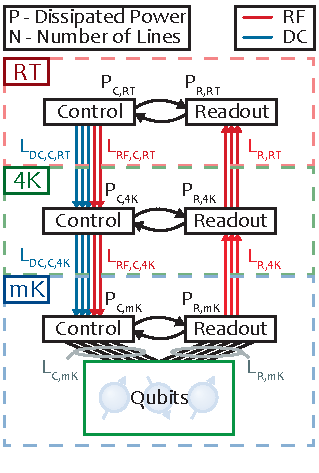
\includegraphics[width=0.5\linewidth]{genarch}
  \caption[Generalized quantum computing architecture]
  {\label{fig:genarch}A generalized qubit architecture, broken into control and readout stages at each temperature stage of a cryostat. The architecture is characterized by number of lines which run between each stage, for example $N_{RF,C,RT}$ for the number of coaxial control lines running from room temperature to the \SI{4}{\kelvin} stage of the cryostat, which will vary depending on the choice of a given architecture. In addition, each stage will dissipate a certain amount of power, for example $P_{R,4K}$ being the power dissipated at \SI{4}{\kelvin} by the readout stage, caused either by active logic, such as an FPGA, amplifiers or off-the-shelf instrumentation, or by passive dissipation, for example due to attenuators.}
\end{figure}

In the remainder of this section, I will quickly review the challenges for control and readout for a large-scale quantum computer, which very much remains
an open question in the field. As we move through the following sections, the sources of many of the numbers in Table~\ref{tab:arch} should become clear
as well as our vision for solving some of these problems. In general, I will progress from the qubit plane up to room temperature control, however this
structure is by no means struct.

\subsection{Control Plane}
A popular refrain for proponents of semiconductor-based qubits is to point to the maturity and flexibilty of modern semiconductor processing as an argument
for the scalability of qubits based on similar processes. While it is undoubtedly true that the miniaturization of transistors has translated into an ability
to fabricate finer devices, the scalability of quantum computers based on such an argument is by no means as clear. The problem, and indeed the main diffrentiator
between a qubit and a transistor, it that while a transistor has the ability to drive other transistors, a qubit has no similar ability. All control of a qubit
must come from outside. This unfortunate fact is captured in Rent's rule, which relates the number of external terminals (or pins) $T$ of an IC, to the number of
internal components (or transistors) $g$:
\begin{equation}
  T = tg^p
  \label{eq:rent}
\end{equation}
where t and p are constants of the system. For an integrated circuit, the value of $p$ generally ranges from 0.5 to 0.8~\cite{5388820}, however for a quantum
circuit, it is reasonably simple to see that this exponent must be 1! Each qubit must be driven by some number $t$ gates, with no qubit able to drive another
qubit without some external control.

The above statement captures the primary difficulty that we will run into when designing qubit chips. While classical ICs can rely on some fan-out to minimize
the number of inputs required, the design of a quantum chip must be able to bring supply high density wiring with high bandwidth and low cross-talk. In addition,
classical CMOS processes usually have only a few layers of high-density interconnect, used only for short-range connections~\cite{5424258}, while qubit
architectures generally require several layers of high-density interconnect over the length of an entire chip~\cite{s41467-017-01905-6}. The question then is
what sets the maximum pitch of a qubit on a chip, as this gives us the density of control lines that must be achieved. Then, given that pitch, how many lines could
we bring in to such a device, given a 1D or a 2D grid of qubits?

The answer to the first question, the pitch of qubit devices, will be set by the length scale over which coupling can be achieved. For spin qubit devices based only
on direct exchange for example, the pitch of qubits will be roughly the size of the qubit itself, as coupling only occurs when electrons can directly tunnel between
neighbouring devices~\cite{PhysRevB.86.085423}. Work presented in this thesis uses elongated many-electron quantum dots to increase this to the micron-scale in
Section~\ref{sec:5dot}, an approach which will likely be applicable majorana devices that use quantum dots as couplers~\cite{PhysRevB.95.235305}. Finally, long
distance coupling of spins via superconducting resonators~\cite{PhysRevB.97.235409} has recently been demonstrated~\cite{2019arXiv190500776B}, enabling coupling
over \si{\milli\meter} length scales.

The next question is how many lines we can bring to a device. In a 1D device geometry, that is for a single line of qubits, the answer is limited only by the
physical size of the chip, and the size of pads (bond pads or bump pads) that we are able to make contact to. For example, a singlet triplet qubit which requires
10 control lines, and pads of pitch $100\times100\si{\micro\meter}$ will require a chip with a \SI{0.01}{\square\milli\meter} area, assuming of course that we are
able to make contact in 3D (i.e. overlapping bonds). In the case that we are only able to make contact in 2D, a chip of size $400\times400\si{\micro\meter}$ at a
minimum is required to break pads out to the edge of a device. The situation is more difficult to evaluate in a 2D array. Firstly, a 2D array is not possible on
a single planar grid, as control lines for inner qubits must be broken out. Therefore a sufficient distance between qubits must be possible to allow control lines
to be brought in from upper layers. To allow fanout of a dense grid leads to a problem very similar to that of routing a BGA package. There will be a relationship
between number of layers, track pitch and via (inter-layer contact) pitch, which will set a hard density limit on qubit devices. Therefore increasing the pitch of
qubit devices via long distance coupling may be necessary when moving to 2D grids. Furthermore, the design of qubit layouts allowing realistic wiring schemes will
continue to be crucial moving forwards~\cite{10.1038/s41534-018-0074-2}. Finally, I point to the potential for multiplexing the control of many qubits onto single
control lines, which may allow the definition of a quantum analog to Rent's rule~\cite{FRANKE20191} (Equation~\ref{eq:rent}). Whether such an architecture is truly
scaleable remains an open question at this time.

While on a single qubit chip, it seems difficult to get around the problem of breaking all control lines out in order to allow qubit control, however, alluding
back to our generalized qubit architecture in Fig.~\ref{fig:genarch}, it should in general be possible to reduce the number of lines running between the 4K stage
and the control plane at mK. To understand why the techniques for doing so, it is useful to separate control pulses into three general forms, microwave excitations,
fast pulses and static confinement. The first two of these require high bandwidth rf wiring, while the latter requires only low bandwidth dc wiring. By the use of
CryoCMOS switches, as detailed in Section~\ref{sec:gooseberry}, it is possible to multiplex a single DC control line to several gates, effectively locking
a voltage onto those gates. Such switches do not dissipate power except when toggled, leading to extremely low power consumption. Similarly, fast pulses may similarly
be generated, again, as detailed in Section~\ref{sec:gooseberry}, minimizing the parasitic capacitance and hence power dissipation, given by $P_\textrm{diss} = CV^2f$
caused by the length of control lines. This leads to the low power consumption of the CryoCMOS architecture in Table~\ref{tab:arch}. The availability of CMOS at low
temperature also gives us a possible solution to the high interconnect density previously discussed, as the pitch of bump-bonding technologies approaches a few \si{\micro\meter}
(with the smallest I am aware of in use at the time of submission being \SI{20}{\micro\meter}~\cite{4550089}). Similarly, the design of low-dissipation and highly integrated
rf-switches as demonstrated in Section~\ref{sec:primelines} allows the routing of a few microwave or pulse lines, which provides a path to further reduction of the footprint
of wiring between stages of the cryostat, as well as a reduction of the signal generation equipment required.

Finally we move up to room temperature, where two primary concerns remain, power consumption and latency (or phase matching), both of which place limits on the footprint
of control electronics at room temperature. In particular, as the rotation rate of qubits is increased, finer tolerances for the phase match of control pulses
is required. When utilizing long control lines, such a phase match is difficult to achieve. Furthermore, as the number of qubits is increased, the footprint of
off-the-shelf electronics, which is in general not designed for simultaneous control of a large number of lines, becomes onerous. In Section.~\ref{sec:primelines}
we address some of these concerns using cryogenic hardware for control, which may allow the use of high density cryogenic interconnects~\cite{Tuckerman_2016}, although
the overall advantages of 4K control require further investigation.

\subsection{Readout}
\label{sec:readout}
In addition to control, the high-fidelity readout of a fragile quantum state is a crucial element of a quantum computer, without which improvements
we make to the control of our qubit are negated. Combining fast, high-fidelity readout with scaleable design complicates the requirements even further,
particularly when we consider the most common desings for readout circuits. As before, I will begin the discussion of readout at the qubit chip level,
and discuss scaleability as we go.

\begin{figure}
  \includegraphics[width=\linewidth]{ReadoutFig}
  \caption[Readout of a semiconductor quantum dot]
  {\label{fig:readout}(a) False color SEM of a five-dot device, similar to the one presented in Sec.~\ref{sec:5dot}. Surface gates are labelled, and
  current is shown running through the charge sensor on the left of the device. (b) Charge sensing signal when the left sensor is tuned as a QPC (1d channel).
  Each step corresponds to a change in the charge occupancy of the quantum dot by 1. (c) Multiplexed readout chip with several resonators, used for
  performing rf readout. (d) Response of the charge sensor in current (right axis) and in reflected rf power (left axis) as the QPC is brought through pinchoff.
  (e) Sample of a charge stability diagram taken using rf charge sensing. Each distinctly coloured region represents a unique charge configuration.}
\end{figure}

For the majority of semiconductor qubit designs, readout is performed via sensing of the charge state of a quantum dot, or quantum dot like
structure. For spin qubits, this is performed by spin-to-charge conversion, where the charge state of a quantum dot will depend on the spin states
of its electrons~\cite{nature02693,PhysRevB.98.125404}, and for Majorana fermions this occurs via the fusion of edge modes (see Sec.~\ref{sec:toporead}).
Typically readout is performed via a proximal charge sensor, which may be formed by a quantum point contact (1D channel), or a sensing dot. A gate pattern
with a sensing dot on the left and right is shown in Fig.~\ref{fig:readout} (a). The conductance of the QPC or sensing dot will depend sensitively
on the charge state of the proximal double quantum dot. This is shown in Fig.~\ref{fig:readout} (b), where steps in the conductance of the QPC correspond to
charges moving on and off the nearby quantum dot. The measurement of this conductance can either be done via a dc lockin measurement or via
rf-reflectometry~\cite{Reilly:2007ig}. The dc measurement is limited by the RC-time constant of the wiring in the fridge, which due to the parasitic
capacitance, filtering and high resistance of the sensor will in general limit bandwidth to a few kilohertz, far greater than the T1 times for spin qubits.
RF measurement is performed by embedding the QPC in a resonator, where the quality factor of the resonator is set by the resistance of the charge sensor.
The derivation of the matching condition is not given here, but I point the interested reader towards~\cite{crootthesis}, where a complete derivation is given.
Of course this immediately points towards the possibility of frequency multiplexing~\cite{doi:10.1063/1.4868107}, allowing the readout of multiple
resonators simultaneously, although the requirement for a proximal charge sensor means such an architecture is unsuitable for 2-D architectures.

\begin{figure}
  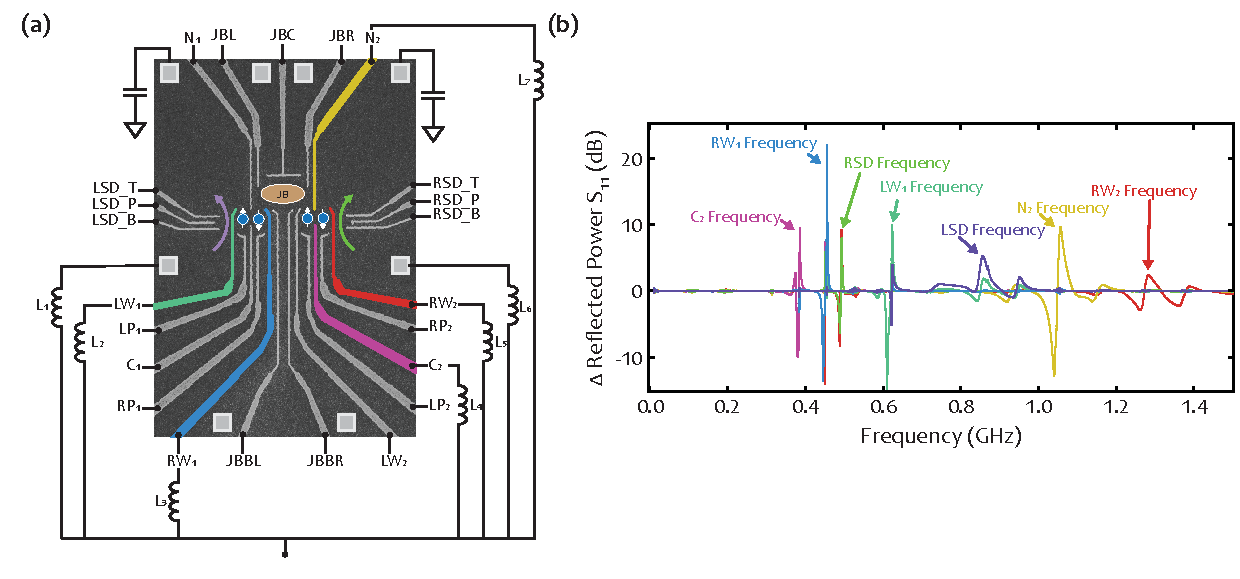
\includegraphics[width=\linewidth]{multifreq}
  \caption[Frequency multiplexed readout of a five-dot device]
  {\label{fig:multifreq}(a) False color SEM of a Five Dot device, identical to the one used in Sec.~\ref{sec:5dot}. A number of resonators are bonded to several gates
  including both charge sensors and dispersive gate sensors. (b) The frequency response of the multiplex chip when the voltage on each gate is changed. Distinct frequencies
  are observed for each gate on the sample.}
\end{figure}

An alternative to using a proximal charge sensor is to use the confining gates themselves as sensors~\cite{PhysRevLett.110.046805}, wherein the quantum capacitance
of the system is measured. The polarizability of a quantum dot is given by:
\begin{equation}
  C_Q = - \diffp[2]{E}{{V_{g}}} = -(\alpha \varepsilon)^2 \diffp[2]{E}{\varepsilon}
\end{equation}
where $\alpha$ is the lever arm and $\varepsilon$ is the tilt, as shown in Fig.~\ref{fig:dqd}. As we can see from the above equation the quantum capacitance
is proportional to the band curvature, which allows us not only to detect charge transitions but also the spin state (since the triplet state has no
curvature at 0 tilt), and hybridization. The latter effect may be used to detect the parity state of a Majorana zero mode coupled to a proximal
quantum dot~\cite{PhysRevB.95.235305}. As with readout via a charge sensor, by embedding a gate in a resonant circuit, we are able to quickly sense changes
in capacitance, with a sensitivity that is sufficient to perform single shot readout of spin states~\cite{fernando1,Nnano_dzurak}. A frequency multiplexed device
with 7 resonators is shown in Fig.~\ref{fig:multifreq}, combining both dispersive and charge-sensing modes of readout.

The potential for frequency multiplexing

\clearpage
\section{Gooseberry}
\label{sec:gooseberry}
%\import{chap2/}{arch}

\clearpage
\section{Cryogenic Control Architecture for Large-Scale Quantum Computing}
\label{sec:primelines}
\import{chap2/}{arch}